\chapter{Calibración de cámaras}\index{Calibracion!de cámara}
\label{cap:calibracion}
La visión comienza con la captura de la luz\ldots

\section{Modelo de cámara Pinhole}\index{Pinhole}
\label{sec:modelo_pinhole}
Una cámara en términos matemáticos es vista\ldots


\begin{figure}
	\centering
  	\begin{tabular}{ccc}
		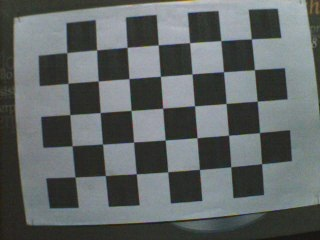
\includegraphics[width=0.3\textwidth]{imagendistorsion.jpg} &
		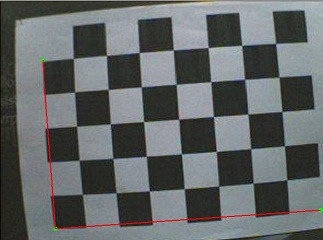
\includegraphics[width=0.3\textwidth]{imagenproceso.jpg} &
		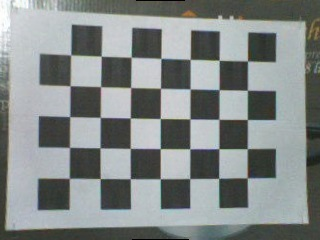
\includegraphics[width=0.3\textwidth]{imagencorregida.jpg} 
 		\\(a) & (b) & (c) 
		\\ 
	\end{tabular}
	\caption{Ejemplo posición de imágenes a tres columnas (a)Imagen con presencia de aberraciones radiales 
	(b) Imagen con selección de una linea para elaborar la corrección (c) Imagen corregida}
	\label{fig:EjemploDistorsion}
\end{figure}

Usualmente siempre va una sección dedicada al análisis y conclusiones adquiridas en el presente capítulo.
\section{Análisis y conclusiones}
En este capítulo se ha descrito el concepto de calibración\ldots